%%%%%%%%%%%%%%%%%%%%%%%%%%%%%%%%%%%%%%%%%%%%%%%%%%%%%%%%%%%%%%%%%%%%%%%%%%%%%%%
%     STYLE POUR LES EXPOSÉS TECHNIQUES
%         3e année INSA de Rennes
%
%             NE PAS MODIFIER
%%%%%%%%%%%%%%%%%%%%%%%%%%%%%%%%%%%%%%%%%%%%%%%%%%%%%%%%%%%%%%%%%%%%%%%%%%%%%%%

\documentclass[a4paper,11pt]{article}

\usepackage{exptech}       % Fichier (./exptech.sty) contenant les styles pour
                           % l'expose technique (ne pas le modifier)


%\linespread{1,6}          % Pour une version destinée à un relecteur,
                           % décommenter cette commande (double interligne)

% UTILISEZ SPELL (correcteur orthographique) à accès simplifié depuis XEmacs


%\setlength{\parskip}{2ex}
\usepackage{color}
\usepackage{graphicx}
\usepackage{hyperref}
\usepackage{ulem}
\hypersetup{
  bookmarks=true,         % show bookmarks bar?
  pdftitle={\'Etude pratique - Data carving},    % title
  pdfnewwindow=true,      % links in new window
  colorlinks=true,       % false: boxed links; true: colored links
  linkcolor=red,          % color of internal links (change box color with linkbordercolor)
  citecolor=green,        % color of links to bibliography
  filecolor=magenta,      % color of file links
  urlcolor=cyan           % color of external links
}
\definecolor{simColor}{rgb}{0.0, 0.5, 0.0}
\definecolor{dissimColor}{rgb}{0.8, 0.0, 0.0}
\definecolor{otherSimColor}{rgb}{0.0, 0.28, 0.67}

%%%%%%%%%%%%%%%%%%%%%%%%%%%%%%%%%%%%%%%%%%%%%%%%%%%%%%%%%%%%%%%%%%%%%%%%%%%%%%%
\normalem
\title{ \textbf{Memory Carving Applied to SmardCard Dumps} }
\markright{\'Etude pratique - Data carving}
                           % Pour avoir le titre de l'expose sur chaque page

\author{Alexandre \textsc{Audinot}, Thierry \textsc{Gaugry}, \\
        Nicolas \textsc{Hurman}, Gabriel \textsc{Prevosto} \\
        \\
        Encadrant : Gildas \textsc{Avoine}}

\date{}                    % Ne pas modifier

%%%%%%%%%%%%%%%%%%%%%%%%%%%%%%%%%%%%%%%%%%%%%%%%%%%%%%%%%%%%%%%%%%%%%%%%%%%%%%%

\begin{document}

\maketitle                 % Génère le titre
\thispagestyle{empty}      % Supprime le numéro de page sur la 1re page



\begin{abstract}
Nous possédons une multitude d'appareils que nous utilisons chaque jour, parfois à notre insu. Quelles informations enregistrent-ils ?
Au cours de cette étude pratique, nous avons essayé de développer un logiciel permettant de comprendre la structure d'une mémoire de petite taille, comme on peut en trouver dans des cartes de transport, des abonnements de ski ou encore dans l'électronique embarquée de nos véhicules. En appliquant une série d'algorithmes et à travers une interface intuitive, disséquer ce type de support devient une tâche plus simple et accessible.
\end{abstract}

\section{Introduction}
  \subsection{Contexte} Dans le cadre du projet \texttt{Études Pratiques} de 3ème année du département informatique, nous avons travaillé sur le sujet « Memory Carving Applied to SmardCard Dumps », avec l'aide de Gildas Avoine qui nous a accompagné tout au long de ce projet. Ce domaine nous étant totalement étranger, nous avons commencé par le découvrir à travers une recherche bibliographique. En partant du \texttt{dump} de la mémoire d'une smartcard, il est possible de retrouver les informations qui y sont contenues, ainsi que la manière dont elles sont structurées.

Les données peuvent être enregistrées de diverses manières suivant leur type. Pour le texte, il existe une multitude d'encodages tels que ASCII ou UTF-8 pour citer les plus connus. Les dates peuvent être sous la forme d'un nombre de secondes écoulées, au format JJ/MM/AAAA et bien d'autres. Devant le nomre de représentations différentes de la même donnée, réaliser un catalogue exhaustif des encodages serait une tâche immense et jamais terminée. Aussi nous nous sommes plus attardés sur une analyse des données permettant de mettre en avant leur structure, ou profitant des informations déjà connues (comme le nom de la personne) pour retrouver l'encodage utilisé et la localisation dans la mémoire du champ donné.

  \subsection{\'Etude de l'existant} L'étude bibliographique que nous avons réalisée ne nous a fourni que peu de pistes vers des travaux existants sur le sujet. En effet, il existe une multitude d'outils de \texttt{data carving}, mais ils sont le plus souvent destinés à de beaucoup plus vastes volumes de données, et en connaissant relativement précisément l'information recherchée (des fichers JPEG sur un disque dur abîmé par exemple). La particularité de notre sujet tient dans le fait que les volumes considérés sont extrèmement faibles, avec une structure qui varie énormément d'un support à l'autre. En effet, étant donné l'espace de stockage disponible sur une \texttt{smartcard}, les entreprises utilisent le plus souvent des structures qui leur sont exclusives.

Nous avons toutefois pu identifier un outil, mCarve \cite{mCarve}, qui illustrait un thème plus général mais correspondait en quelques points à ce que nous recherchions. Le défaut principal de mCarve est qu'il est essentiellement basé sur une analyse dynamique de dumps, où l'on possède plusieurs versions du même fichier capturées à des instants différents. Notre sujet portant également sur des analyses statiques, il fallait y ajouter un bon nombre de fonctionnalités. De plus, nous l'avons trouvé relativement peu intuitif à l'usage, l'interface utilisateur ne présentant que les résultats bruts des algorithmes de comparaison.

\section{Cahier des charges}
  Lors de l'étude préliminaire du projet, nous avions établi un cahier des charges. Voici un tableau récapitulatif du travail accompli par rapport au résultat attendu.
\paragraph{}

\begin{tabular}{|p{6cm}|p{6cm}|}
  \hline
  Permettre à l'utilisateur d'extraire des données d'un dump de mémoire de petite taille et de structure inconnue &
  L'utilisateur peut trouver des informations en appliquant différents encodages à un dump quelle que soit sa structure
  \\ \hline
  Être utilisable sur un dump unique ou sur un ensemble de dumps &
  L'application permet de créer des ensembles de dumps qui regroupent un ou plusieurs dumps
  \\ \hline
  Donne la possibilité à l'utilisateur de garder une trace des données déjà extraites &
  Le travail peut être enregistré sous forme de masque
  \\ \hline
  Traduire le binaire vers différents encodages et vice versa &
  L'utilisateur peut choisir comment afficher le dump courant parmi une liste d'encodages
  \\ \hline
  Fonctionne sous windows et linux &
  Le programme a été testé et fonctionne sous les deux environnements
  \\ \hline \hline
  \textbf{Optionnel} &
  \\ \hline
  Donne une représentation visuelle des données grâce à un code couleur &
  Une vue bitmap affiche les données sous forme binaire avec des couleurs pour une meilleur lisibilité
  \\ \hline
  Permet à l'utilisateur de créer des masques et de les réutiliser &
  Enregistrement du travail sous forme de masques
  \\ \hline
  Peut reconnaître les images dans les dumps &
  Objectif non achevé par manque de temps
  \\ \hline
\end{tabular}

\section{Présentation du logiciel}
  \subsection{Technologies utilisées} Pour réaliser ce projet, nous avons utilisé un langage et des librairies multi-plateformes comme imposé par le cahier des charges. Le logiciel est écrit en C++, avec la librairie Qt \cite{Qt} pour l'interface graphique.

Un framework de tests unitaires, UnitTest++ \cite{UnitTest}, a également été mis en place pour tester les composants clé du logiciel. Doxygen \cite{Doxygen} nous a permis de générer la documentation technique.

Nos recherches ne nous ont ni permi de trouver des librairies de manipulation de chaînes de bits répondant à nos attentes, ni des implémentations des algorithmes utilisés satisfaisantes. Nous avons donc dû en écrire nos propres versions.

  \subsection{Interface} L'interface utilisateur est découpée en 3 parties, qui reprennent les trois fonctionnalités clé du logiciel.

\begin{figure}[!h]
  \begin{center}
  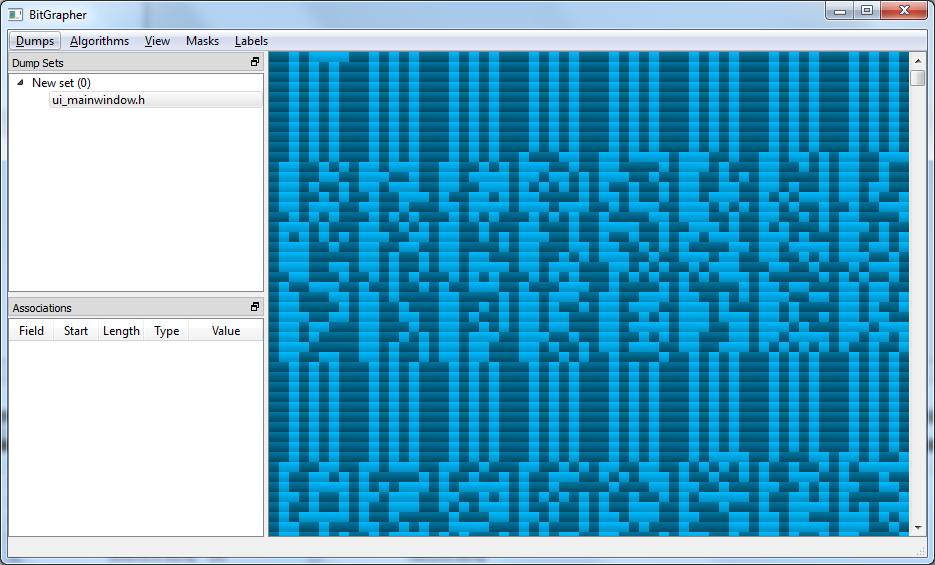
\includegraphics[width=\textwidth]{res/03-2-interface.png}
  \caption{Interface du logiciel}
  \label{03-2-interface}
  \end{center}
\end{figure}

Le premier volet, en haut à gquche, contient la liste des \texttt{dump sets} actuellement étudiés. Un dump set peut contenir plusieurs dumps, qui seront comparés entre eux.

Le second volet, en bas à gauche, affiche la liste des champs identifiés par l'utilisateur. Au fur et à mesure de l'analyse du dump, les données collectées permettent de comprendre la structure du fichier.

La zone d'affichage princpale, à droite, correspond à une visualisation des données du dump, qui peut être sous la forme de bitmap comme sur l'image, ou bien sous forme textuelle avec un encodage choisi au préalable.

Les menus donnent accès aux différents outils d'analyse, ainsi qu'à la sauvegarde et au chargement de dumps, de dumpsets ou de masques.

L'interface utilisateur est entièrement fluide et les volets peuvent être détachés ou déplacés pour que l'utilisateur puisse organiser son espace de travail comme il le souhaite.

  \subsection{Fonctionnalités} \begin{description}
  \item[Dump sets] \hfill \\
  Les dumps chargés sont regroupés en dump sets. Un dump set représente plusieurs versions de la même mémoire, ou bien des mémoires similaires. Des opérations peuvent être appliquées sur les dump sets pour comparer les dumps.

  \item[Similarities] \hfill \\
  Recherche des similitudes entre plusieurs dumps.

  \item[Dotplot pattern] \hfill \\
  Analyse visuelle des motifs récurrents.

  \item[Masks] \hfill \\
  Enregistrement de la structure d'un dump. Une fois l'analyse d'un dump terminée, il est possible de l'enregistrer dans un fichier \texttt{.mk} et de la recharger plus tard pour l'appliquer à un autre dump suivant le même format et directement avoir accès aux différents champs.

  \item[Labels] \hfill \\
  Association d'une zone de données du dump à un encodage et une étiquette. Notre logiciel prend en charge les encodages les plus courants, en traduisant les bits composant le dump de différentes manières suivant le type du champ considéré.
\end{description}

\section{Algorithmique}
  \subsection{Analyse des dumps} \label{04-analyse} Cet outil permet d'appliquer plusieurs algorithmes aux dumps, afin d'aider au repérage de l'information recherchée.

\subsubsection{Similarities \cite {ref-vandeursen}} \label{04-similarities}

Cet algorithme permet de mettre en évidence, dans un groupe de dumps, les chaînes de bits semblables (que nous appellerons similarités) ou dissemblables (que nous appellerons dissimilarités). Ces chaînes doivent être au même endroit dans chaque dump pour être reconnues.

Dans le cas de deux dumps, les similarités sont représentées par la couleur verte, tandis que les similarités sont représentées par la couleur rouge.

\begin{figure}[!h]
  \begin{center}
  {\tt\center
  {\color{simColor} Ce}{\color{dissimColor} ci es}{\color{simColor}t }{\color{dissimColor} un exemple de }{\color{simColor} similarité}

  {\color{simColor} Ce}{\color{dissimColor} la me}{\color{simColor}t }{\color{dissimColor} en couleur la }{\color{simColor} similarité}
  }
  \end{center}
  \caption{Exemple de similarités}
  \label{04-1-sim_simple}
\end{figure}

Afin d'affiner la recherche, il est possible de spécifier une taille de chaîne minimum :

\begin{figure}[!h]
  \begin{center}
  {\tt
  {\color{dissimColor} Ceci est un exemple de }{\color{simColor} similarité }{\color{dissimColor} avec une taille minimum de 4}

  {\color{dissimColor} Cela met en couleur la }{\color{simColor} similarité }{\color{dissimColor} faisant plus de 4 caractères}
  }
  \end{center}
  \caption{Similarités avec une taille de chaîne minimum}
  \label{04-1-sim_taille_min}
\end{figure}


Dans le cas de plusieurs dumps, on dispose de trois couleurs. Le rouge représente les dissimilarités, le vert les similarités concernant le dump visualisé (c'est-à dire les similarités commune à ce dump et à d'autres), tandis que le bleu correspond aux similarités ne concernant pas le dump visualisé (c'est-à dire les similarités communes à d'autres dumps).
Ces couleurs ont des nuances : plus le vert ou le bleu sont prononcés, plus il y a de dumps partageant la similarité en question.

\begin{figure}[!h]
  \begin{center}
  {\tt
  {\color{dissimColor} Encore un}{\color{otherSimColor} e au}{\color{dissimColor} tre }{\color{simColor} similarité}{\color{dissimColor} .}

  {\color{dissimColor} Toujours }{\color{simColor} plus }{\color{dissimColor} de }{\color{simColor} similarité}{\color{dissimColor} s}

  {\color{dissimColor} colorées }{\color{simColor} plus }{\color{dissimColor} qu'}{\color{otherSimColor} auparavant}{\color{dissimColor} .}
  }
  \end{center}
  \caption{Similatités entre trois dumps}
  \label{04-1-sim_mult}
\end{figure}

\subsubsection{Dotplot patterns \cite {ref-dotplot}} \label{04-dotplot}

Cet algorithme s'applique à deux dumps et génère un schéma similaire à celui ci-dessous :

\begin{figure}[!h]
  \begin{center}
  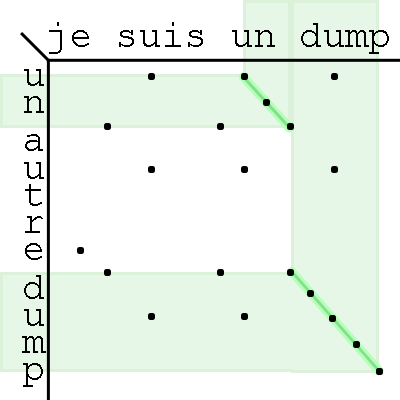
\includegraphics[scale=1]{res/04-2-dotplot.png}
  \caption{Un motif obtenu par dotplot}
  \label{04-1-dotplot}
  \end{center}
\end{figure}

Sur ce schéma, on retrouve l'un des dumps en abscisse, et l'autre en ordonnée. Les diagonales représentent des chaînes de bits semblables dans les deux dumps qui, contrairement aux similarités, ne sont pas nécessairement au même emplacement dans chaque dump. Leurs coordonnées représentent leurs positions dans chacun des dumps.

Dans cet exemple, on constate deux diagonales : l'une correspondant à la répétition du mot \texttt{un}, l'autre, plus longue, à celle du mot \texttt{dump}.

  \subsection{Complexité} La complexité de nos algorithmes est la suivante :

\begin{itemize}
  \item Pour les dotplot patterns, une complexité en $O(t^{2})$ où $t$ est la taille du ou des dump(s) en bits.
  \item Pour les similarités, une complexité en $O(n^{2}\times t)$ où $n$ est le nombre de dumps et $t$ la taille des dumps en bits.
\end{itemize}

  \subsection{Aide à la décision} Afin de mieux assister l'utilisateur dans son analyse, des aides à la décision ont été implémentées.

\subsubsection{Formats d'entrée}

Tout d'abord, lors de l'ouverture d'un dump, l'aide à la décision sélectionne le format le plus probable parmi binaire, hexadécimal ou donnée brute. L'utilisateur a tout de même le choix parmi les autres formats, à part ceux qui ne sont pas respectés par le fichier en entrée.
Par exemple, si l'on tente d'ouvrir un fichier contenant la chaîne ASCII ''0A1F'', l'aide à la décision la reconnaîtra comme de l'hexadécimal. L'utilisateur pourra également choisir l'option ''données brutes'', qui importe les caractères ASCII directement, mais pas l'option binaire, la chaîne contenant autre chose que des ''0'' et des ''1'.

\subsubsection{Tailles de chaîne minimale pour l'analyse}

Ensuite, lors de l'application d'un algorithme de comparaison de dumps (voir Section \ref{04-analyse}), une taille de chaîne à comparer minimale est demandée à l'utilisateur. Par la simple pression d'un bouton, cette valeur peut être sélectionnée automatiquement par le programme en fonction de la taille et du nombre de dumps à comparer.
Ces valeurs automatiques ont été calculées afin de donner une probabilité d'obtenir un résultat par hasard (qui serait donc un faux positif) d'au plus 5\%.

Pour simplifier les calculs, nous avons établi les hypothèses suivantes :
\begin{itemize}
	\item Ne connaissant pas par avance leur structure, nous avons supposé une distribution aléatoire des bits dans les dumps.
	\item Nous avons supposée la taille des dumps en bits grande par rapport à 1. Dans la pratique, cette taille sera de quelques Ko.
	\item Nous avons supposé le nombre de dumps négligeable devant leur taille en bits. Cela ne devrait pas poser de problème, car le nombre de dumps par set est au plus de l'ordre de la dizaine.
\end{itemize}
Nos résultats indiquent les tailles de chaînes minimales suivantes, pour deux dumps de 1Ko :
\begin{itemize}
	\item 18 bits pour l'algorithme des similarités (Voir Section \ref{04-similarities}).
	\item 31 bits pour l'algorithme des dotplot patterns (Voir Section \ref{04-dotplot}).
\end{itemize}
\section{Gestion du projet}
  \subsection{Outils}

Dans le cadre de ce projet, nous avons mis en place diverses méthodes et outils de travail en groupe. Nous avons par exemple utilisé des outils de travail collaboratif pour partager nos ressources et mettre notre travail en commun :
\begin{itemize}
        \item Git : outil de versionnage pour partager le code source de notre application ;
        \item Google Drive : système de stockage et synchronisation de fichiers pour tous les autres documents de notre projet.
\end{itemize}

\subsection{Organisation}

Nous nous sommes régulièrement réunis avec notre encadrant pour discuter de l’avancement du projet ainsi que des futures fonctionnalités à implémenter. Nous avons également effectué des réunions sans notre encadrant pour séparer notre projet en plusieurs tâches et pouvoir répartir le travail. Nous avons ainsi choisi des tâches indépendantes les unes des autres pour que chacun puisse travailler dessus en même temps.

Dans le but de nous assurer de l'avancement de notre projet, nous avons fixé des dates pour plusieurs versions intermédiaires de notre logiciel. Cependant, à cause du retard accumulé, une seule version intermédiaire a pu être produite.

Notre encadrant a suggérée que chaque membre du groupe relève ses temps de travail pour qu'à la fin du projet, il soit possible d'identifier les tâches qui nous ont pris le plus de temps.


\section{Améliorations envisageables}
  Nous avons réalisé notre logiciel pour répondre à la problématique qui nous était posée, et n'avons pas eu le temps d'implémenter d'autres fonctionnalités ; certaines nous sembleraient cependant réellement utiles.

\begin{description}
  \item[Optimisations] \hfill \\
  Nous n'avons pas réalisé de tests de performances avec des outils de profiling.
  Il serait judicieux de le faire, en particulier sur les algorithmes, ce qui pourrait permettre de diviser le temps nécessaire à l'analyse des dumps. En effet, certains de nos algorithmes ont une complexité qui n'est peut-être pas la meilleure.

  \item[Masques préchargés] \hfill \\
  Il serait utile de réaliser un ensemble de masques livrés avec le logiciel permettant d'ouvrir des dumps provenant des cartes les plus répandues sans avoir à refaire le travail d'analyse.

  \item[Environnement plus intégré] \hfill \\
  Actuellement, plusieurs outils sont nécessaires : un pour l'extraction du dump depuis la carte, un second pour analyser le dump et éventuellement un troisième pour mettre en forme les résultats. Intégrer les fonctionnalités de notre logiciel dans un environnement permettant de réaliser l'ensemble de la procédure à travers la même interface apporterait une meilleure expérience utilisateur.

  \item[Davantage de visualisations] \hfill \\
  Certains types de données, comme les images, ne sont pas prises en charge par notre logiciel. Pour certaines mémoires, comme celles des passeports, ce type de visualisation serait intéressant.

  \item[Plugins pour les encodages] \hfill \\
  Nous avons volontairement limité le nombre d'encodages pris en charge, pour ne pas perdre de temps et pouvoir nous concentrer sur des fonctionnalités plus intéressantes. Pouvoir exporter les encodages dans des fichiers séparés permettrait à chaque utilisateur de définir son encodage s'il n'existe pas déjà et de les partager.

  \item[Traduire le logiciel] \hfill \\
  L'interface a été réalisée en anglais, une internationalisation la rendrait plus conviviale pour les différents utilisateurs.
\end{description}

%\newpage
\bibliography{biblio}

\end{document}
